\documentclass[11pt]{article}

\usepackage[margin=1in]{geometry}
\usepackage{amsmath,amssymb,amsthm}
\usepackage{array}
\usepackage{booktabs}
\usepackage{enumitem}
\usepackage{float}
\usepackage{graphicx}
\usepackage{hyperref}
\usepackage[numbers]{natbib}
\usepackage{tikz}
\usepackage{titlesec}
\usepackage{xcolor}
\usetikzlibrary{arrows.meta,calc,fit,positioning,shapes.geometric}

\titleformat{\section}{\normalfont\Large\bfseries}{\thesection}{1em}{}
\titleformat{\subsection}{\normalfont\large\bfseries}{\thesubsection}{1em}{}
\titleformat{\subsubsection}{\normalfont\normalsize\bfseries}{\thesubsubsection}{1em}{}
\titleformat{\paragraph}{\normalfont\small\itshape}{\theparagraph}{1em}{}
\titlespacing*{\section}{0pt}{3.5ex plus 1ex minus .2ex}{2.3ex plus .2ex}
\titlespacing*{\subsection}{0pt}{3.25ex plus 1ex minus .2ex}{1.5ex plus .2ex}
\titlespacing*{\subsubsection}{0pt}{3.25ex plus 1ex minus .2ex}{1.5ex plus .2ex}
\titlespacing*{\paragraph}{0pt}{2.5ex plus 1ex minus .2ex}{1ex plus .2ex}
\setlength{\parindent}{0pt}
\setlength{\parskip}{6pt}

\theoremstyle{definition}
\newtheorem{definition}{Definition}[section]

\title{Octopus CXL Memory Pooling:\\Current Status, Failure Analysis, and RL Redesign}
\author{Pulak Mehrotra}
\date{March 2026}

\begin{document}
\maketitle

\begin{abstract}
Octopus is a sparse CXL memory-pooling architecture in which each server can draw
memory only from a limited neighborhood of multi-ported devices (MPDs). The
systems opportunity is clear: production cloud traces exhibit persistent
peak-to-mean gaps, so pooling can reduce required memory capacity if allocation
keeps the per-MPD peak low. The challenge is that Octopus is not a generic
load-balancing problem. Sparse topology, long-lived allocations, and
non-migratory decisions couple present placement choices to future congestion.
This report summarizes the current Octopus RL effort in a systems-report format.
It formalizes the problem, documents the current simulator and learning setup,
records the strongest results and failure signals available today, and proposes a
validation-first next-step plan. The main conclusion is that the current failure
mode is a learnability problem, not yet an online adaptation problem: the policy
must first learn balanced offline allocation before methods such as LCPO are
introduced for deployment-time drift.
\end{abstract}

\tableofcontents
\newpage

\section{Motivation}

The motivation for Octopus is economic and operational. Main memory is a major
component of server cost, yet cloud fleets are provisioned for local peaks that
are not synchronized across servers. CXL-based pooling exploits that mismatch by
moving some memory capacity into a shared pool that can absorb temporal and
spatial variation in demand \cite{pond2023}. If the shared pool is allocated
well, required capacity tracks aggregate demand rather than the sum of per-host
worst cases.

The current project evidence points to a real pooling opportunity before any
reinforcement learning claim is made:
\begin{itemize}[nosep]
    \item Azure traces used in this project show clear diurnal structure across
    ten datacenters.
    \item The cluster-level peak-to-mean ratio is roughly $1.13\times$ to
    $1.26\times$, leaving non-trivial recoverable headroom.
    \item Prior Octopus analyses in this codebase already indicate that practical
    sparse topologies can comfortably exceed the rough $3\%$ break-even threshold
    discussed in the project.
\end{itemize}

Figure~\ref{fig:motivation_peak_to_mean} captures the central intuition: the
pooling opportunity exists because aggregate demand is smoother than individual
server demand.

\begin{figure}[H]
\centering
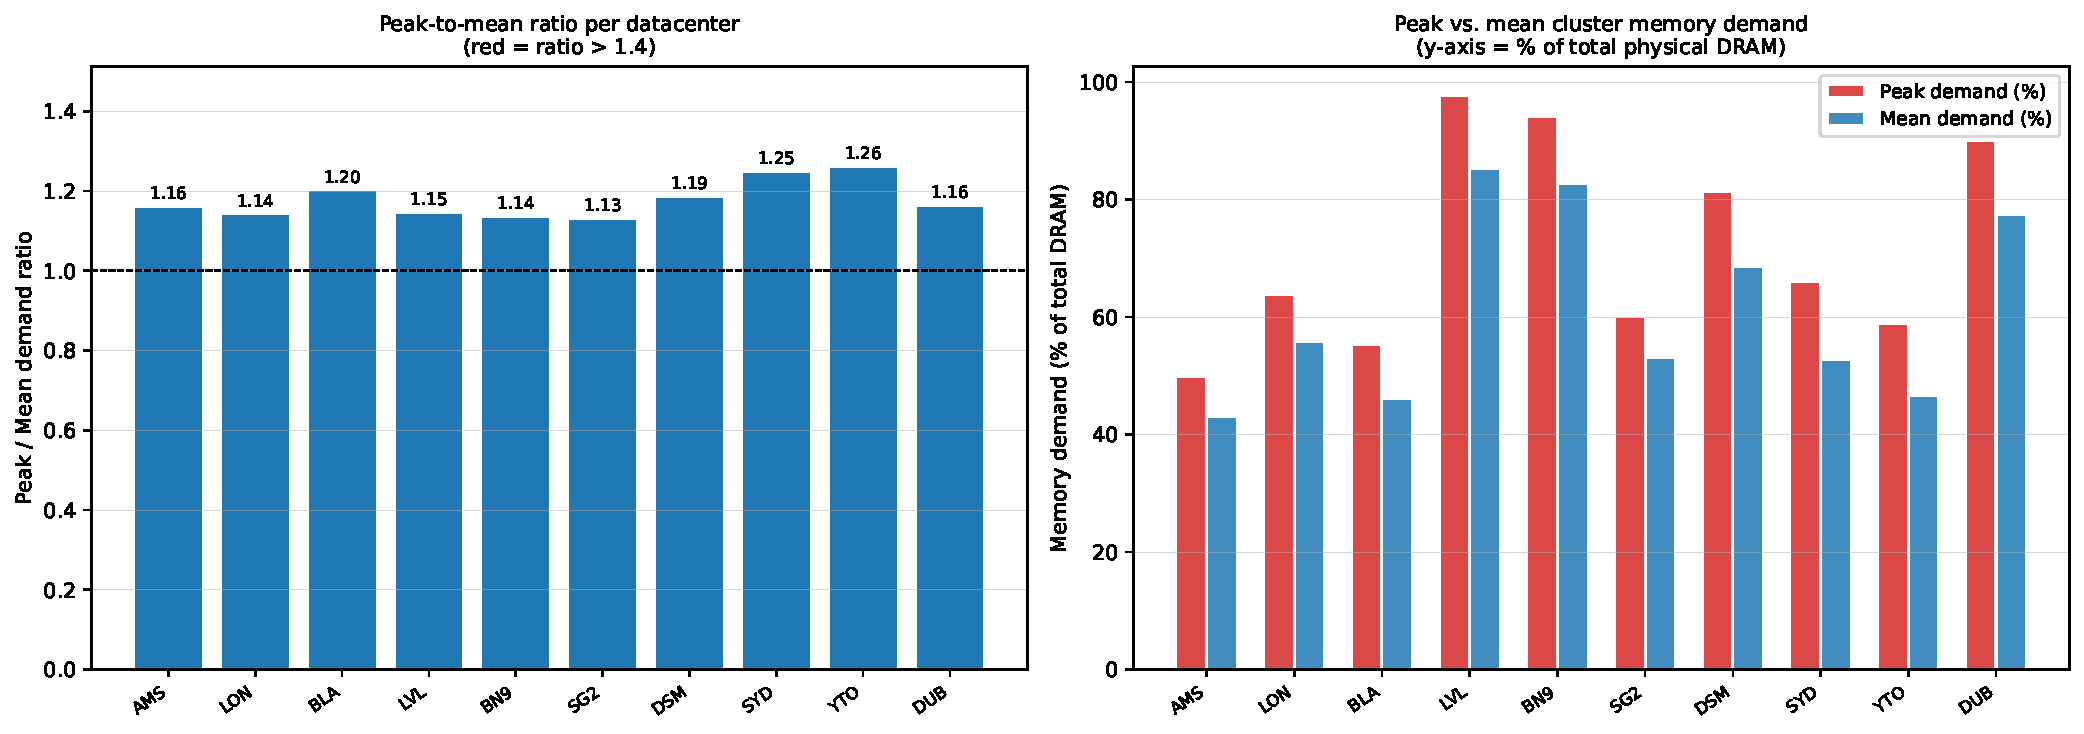
\includegraphics[width=0.92\textwidth]{../v1/figs/peak_to_mean.pdf}
\caption{Peak-to-mean demand evidence from the existing Octopus analysis. The
gap between mean and peak demand is the capacity headroom that pooling tries to
recover.}
\label{fig:motivation_peak_to_mean}
\end{figure}

What makes Octopus interesting from a systems perspective is that pooling alone
is not enough. The architecture deliberately uses sparse connectivity instead of
full crossbar-style reachability. That choice reduces hardware cost, but it
turns memory placement into an online constrained-allocation problem in which a
bad early placement can leave too little headroom for later arrivals.

\section{Problem Statement}

\subsection{Octopus Setting}

Octopus connects servers and MPDs as a sparse bipartite graph. A server can only
place a VM's remote memory on MPDs to which it has physical CXL links. In other
words, topology is part of the problem formulation, not a detail of the
implementation.

\begin{figure}[H]
\centering
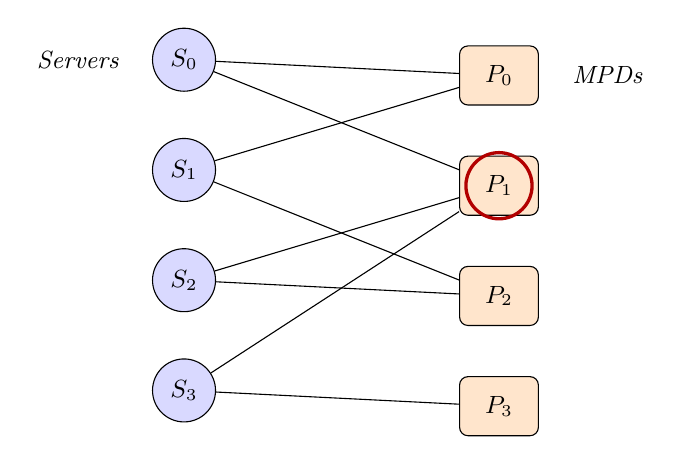
\begin{tikzpicture}[
    >=Stealth,
    every node/.style={font=\small},
    host/.style={draw, circle, fill=blue!15, minimum size=0.8cm},
    mpd/.style={draw, rectangle, rounded corners=3pt, fill=orange!20,
        minimum width=1.0cm, minimum height=0.75cm, align=center}
]
    \node[host] (h0) at (0,2.2) {$S_0$};
    \node[host] (h1) at (0,0.8) {$S_1$};
    \node[host] (h2) at (0,-0.6) {$S_2$};
    \node[host] (h3) at (0,-2.0) {$S_3$};

    \node[mpd] (p0) at (4,2.0) {$P_0$};
    \node[mpd] (p1) at (4,0.6) {$P_1$};
    \node[mpd] (p2) at (4,-0.8) {$P_2$};
    \node[mpd] (p3) at (4,-2.2) {$P_3$};

    \draw (h0) -- (p0);
    \draw (h0) -- (p1);
    \draw (h1) -- (p0);
    \draw (h1) -- (p2);
    \draw (h2) -- (p1);
    \draw (h2) -- (p2);
    \draw (h3) -- (p1);
    \draw (h3) -- (p3);

    \draw[red!70!black, very thick] (p1) circle (0.42);

    \node[font=\small\itshape, left=0.3cm of h0] {Servers};
    \node[font=\small\itshape, right=0.3cm of p0] {MPDs};
\end{tikzpicture}
\caption{Illustrative Octopus topology. A hot subset of servers can collide on a
small MPD neighborhood, so local placement decisions can create future global
bottlenecks.}
\label{fig:octopus_topology}
\end{figure}

\subsection{Allocation Objective}

At each VM arrival on server $S_i$, the allocator receives a request for $x$ GB
of pooled memory and must split that request across the server's reachable MPDs.
Once placed, memory is effectively pinned for the VM lifetime in the current
setup; there is no cheap migration loop that can continuously rebalance past
mistakes.

\begin{definition}[Arrival-Time Allocation Policy]
Let $M \in \{0,1\}^{n \times m}$ be the server-to-MPD adjacency matrix, where
$M_{ij} = 1$ if server $i$ can allocate from MPD $j$. For a VM of size $x$
arriving at server $i$, an allocation policy emits a non-negative vector
$\mathbf{a} \in \mathbb{R}_{\ge 0}^{m}$ such that
\begin{equation}
    \sum_{j=1}^{m} a_j = x,
    \qquad
    a_j = 0 \text{ whenever } M_{ij} = 0.
\end{equation}
\end{definition}

The project metric is pooling savings, defined by the peak load placed on the
worst MPD over the trace horizon:
\begin{equation}
    \text{Pooling Savings}
    =
    1 -
    \frac{m \cdot \max_{j \in [m]}\{\text{PeakLoad}_j\}}
         {\sum_{i=1}^{n} \text{DRAM}_i}.
\end{equation}

This definition matters operationally because all MPDs in a pod are provisioned
symmetrically. The single hottest MPD therefore sets the required capacity, and
the required capacity sets hardware cost.

\subsection{Why the Problem Is Hard}

The current report emphasizes five systems-facing difficulties:
\begin{itemize}[nosep]
    \item \textbf{Sparse topology.} Each server can only use a small neighborhood
    of MPDs, so global balance cannot be assumed.
    \item \textbf{Long-lived effects.} A placement that looks harmless now can
    block headroom many hours later.
    \item \textbf{Online decisions.} Allocation is made at VM arrival time rather
    than by solving a global offline remapping problem.
    \item \textbf{Limited observability.} The agent must infer future congestion
    from partial current state.
    \item \textbf{Generalization.} A policy trained on one trace or one topology
    variant must still behave sensibly on others.
\end{itemize}

These properties explain why this is not simply a matter of ``pick the least
loaded MPD'' and why a learning-based approach remains attractive despite the
current failures. Prior systems work also provides precedent for learned control
policies in resource management, including RL for storage allocation and temporal
pattern exploitation \cite{fleetio2025,coach2025}.

\section{Current Implementation}

The current code path implements an offline RL simulator around VM trace replay.
Each episode replays a real trace, remaps servers to a pod instance, and applies
an allocation policy at every VM arrival. Evaluation is repeated over many random
pod mappings so the reported result is a distribution rather than one
cherry-picked run.

\subsection{Execution Pipeline}

\begin{figure}[H]
\centering
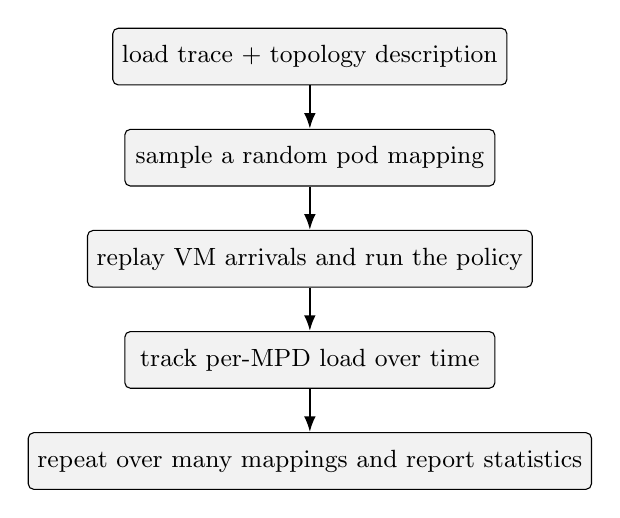
\begin{tikzpicture}[
    node distance=0.55cm,
    box/.style={draw, rounded corners=2pt, minimum width=4.7cm,
        minimum height=0.72cm, align=center, fill=black!5, font=\small},
    arr/.style={-{Latex[length=2mm]}, thick}
]
    \node[box] (trace) {load trace + topology description};
    \node[box, below=of trace] (map) {sample a random pod mapping};
    \node[box, below=of map] (sim) {replay VM arrivals and run the policy};
    \node[box, below=of sim] (peak) {track per-MPD load over time};
    \node[box, below=of peak] (agg) {repeat over many mappings and report statistics};
    \draw[arr] (trace) -- (map);
    \draw[arr] (map) -- (sim);
    \draw[arr] (sim) -- (peak);
    \draw[arr] (peak) -- (agg);
\end{tikzpicture}
\caption{Current Octopus evaluation pipeline. The systems metric is peak
per-MPD capacity under trace replay, aggregated over repeated random pod
mappings.}
\label{fig:implementation_pipeline}
\end{figure}

\subsection{Policy, State, and Reward Today}

Table~\ref{tab:current_impl} summarizes the present implementation focus. The
important point is that the current system already has a usable experimental
skeleton; the bottleneck is policy quality, not lack of simulation machinery.

\begin{table}[H]
\centering
\small
\renewcommand{\arraystretch}{1.25}
\begin{tabular}{p{0.22\linewidth}p{0.70\linewidth}}
\toprule
\textbf{Component} & \textbf{Current implementation} \\
\midrule
Environment & VM-trace replay with random pod remapping per episode; no routine migration after placement. \\
Observation & Reachable MPD loads, connectivity mask, incoming VM size, global peak load, and hour-of-day encoding. \\
Action & Continuous weight vector over reachable MPDs; weights are normalized into an allocation split. \\
Reward & Immediate peak-oriented reward with limited shaping; most signal comes from the current worst MPD. \\
Learner & SAC in Stable-Baselines3 \cite{haarnoja2018sac,stable_baselines3}. \\
Training regime & Current headline runs use 1M timesteps, with a slower and a faster training configuration. \\
Evaluation & Repeated random pod mappings; report average, min, max, and standard deviation of pooling savings. \\
\bottomrule
\end{tabular}
\caption{Current implementation summary. The main issue is not missing
infrastructure, but that the present state and reward do not yet induce the
desired load-balancing behavior.}
\label{tab:current_impl}
\end{table}

\subsection{Current Diagnosis}

The current slides and design notes converge on one diagnosis: the agent is being
asked to solve a hard long-horizon topology-aware problem with insufficient
signal. In particular:
\begin{itemize}[nosep]
    \item the state is too instantaneous and hides future pressure,
    \item the reward is too sparse and mostly scores the current worst MPD,
    \item the training budget is too small relative to the horizon, and
    \item the current train/eval setup is not diverse enough to establish
    generalization.
\end{itemize}

This framing matters because it changes the order of work. The first question is
not whether LCPO should replace SAC. The first question is whether the offline
task has been formulated in a way that is actually learnable.

\section{Current Results}

The current results are best read as a mixed status report rather than a claim of
end-to-end success. The project already demonstrates that pooling is worthwhile
and that the simulation pipeline can expose topology-sensitive behavior. However,
the learned allocator does not yet beat simple baselines.

\subsection{Headline Takeaways}

\begin{itemize}[nosep]
    \item \textbf{The opportunity is real.} Trace data shows enough aggregate
    headroom to justify memory pooling as a systems optimization target.
    \item \textbf{Topology matters.} Sparse Octopus topologies underperform
    fully-connected pooling in prior simulation evidence, confirming that the
    allocation policy has real work to do.
    \item \textbf{The current learned policy fails visibly.} The strongest failure
    signal is approximately $20\times$ max/min MPD imbalance under the current
    SAC policy.
    \item \textbf{Generalization is still weak.} Current proxy training rewards do
    not demonstrate robust improvement on the systems metric of interest.
\end{itemize}

\subsection{Current Failure Signal}

Figure~\ref{fig:current_failure} is the most important present result. Greedy is
not optimal, but it at least behaves like a load balancer. The current SAC
policy, in contrast, concentrates memory onto a small number of MPDs and leaves
others nearly idle.

\begin{figure}[H]
\centering
\begin{minipage}[t]{0.48\textwidth}
\centering
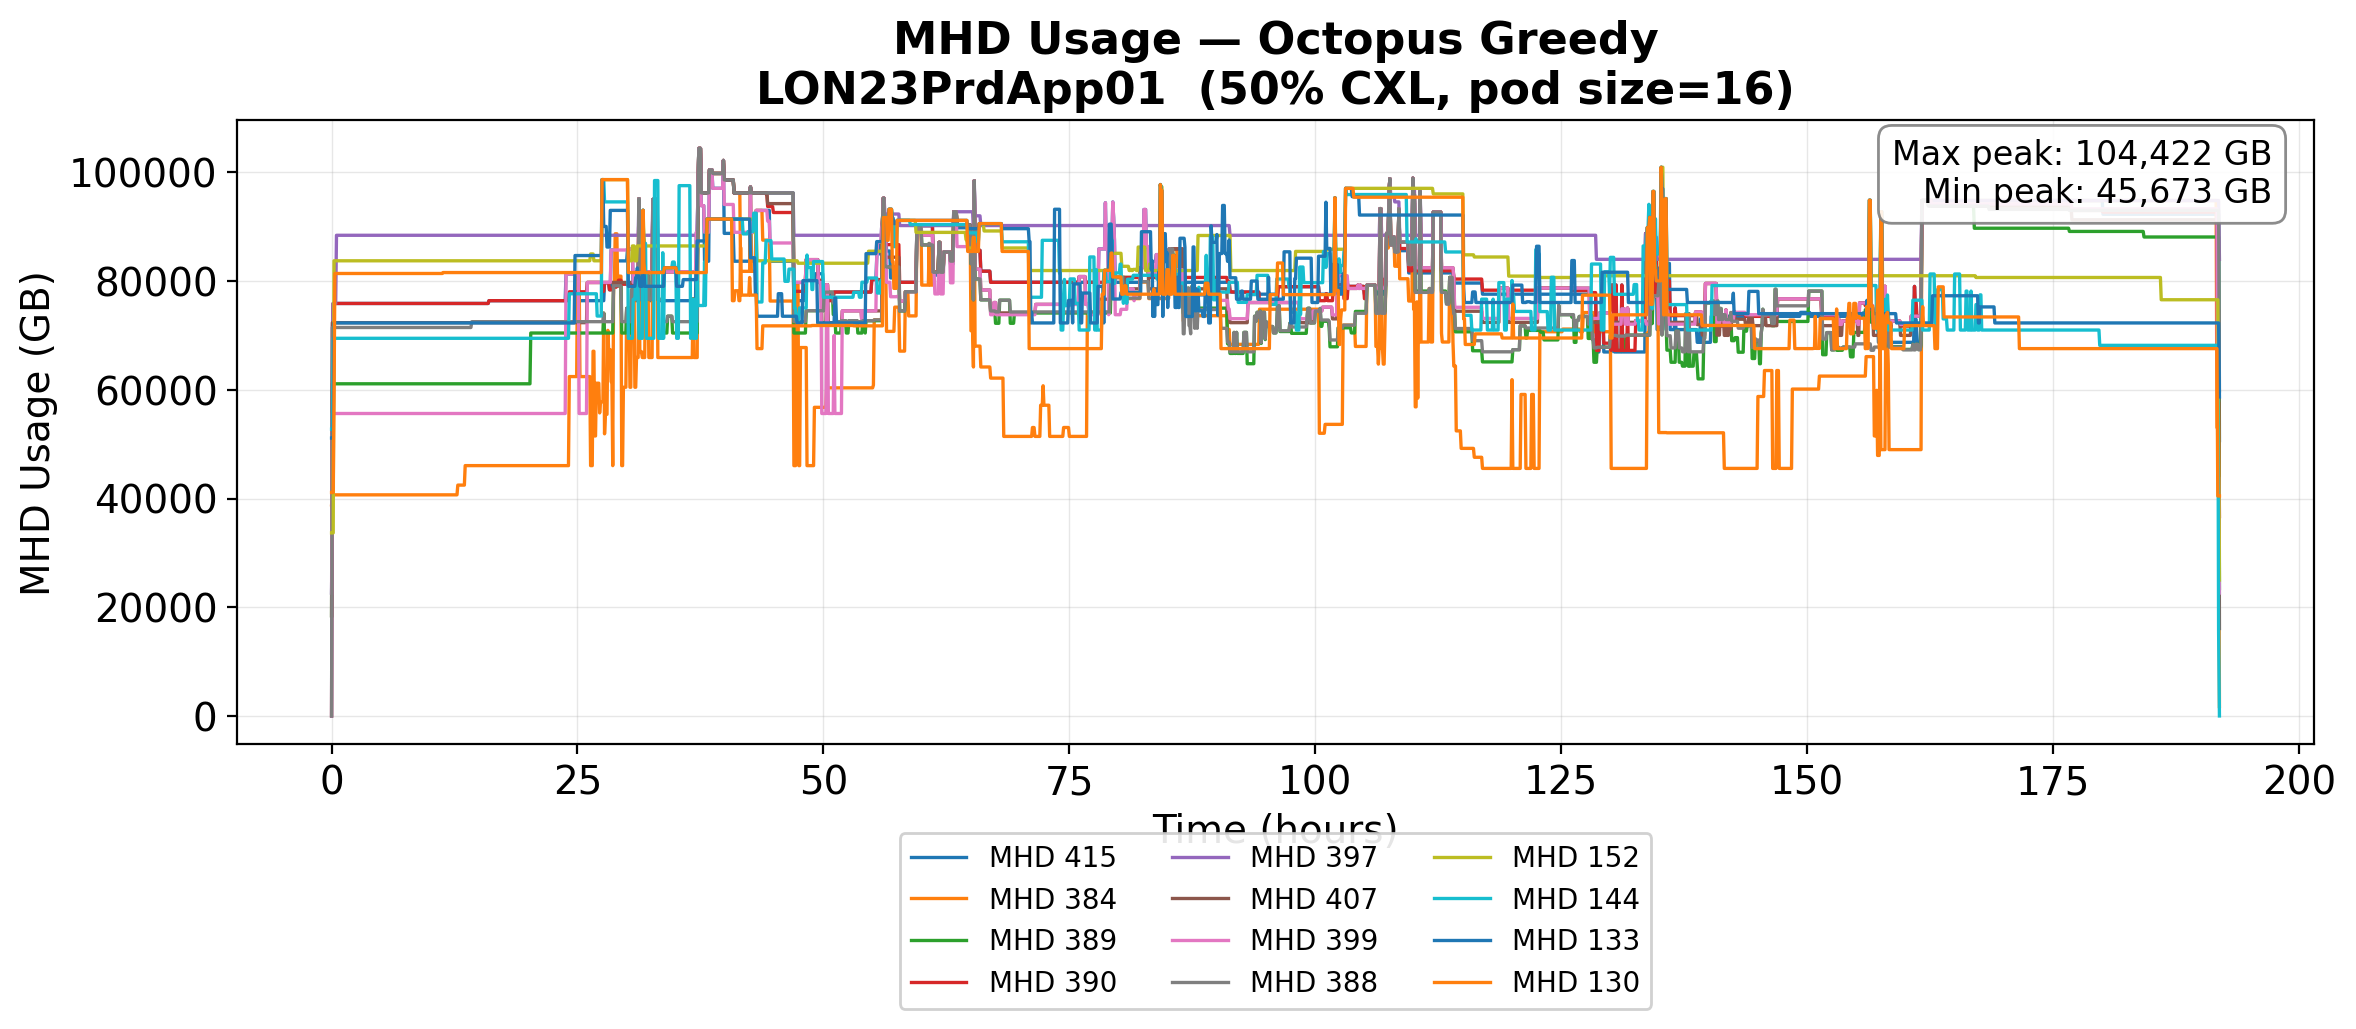
\includegraphics[width=\linewidth]{../v1/figs/mhd_timeseries_greedy.png}
\end{minipage}
\hfill
\begin{minipage}[t]{0.48\textwidth}
\centering
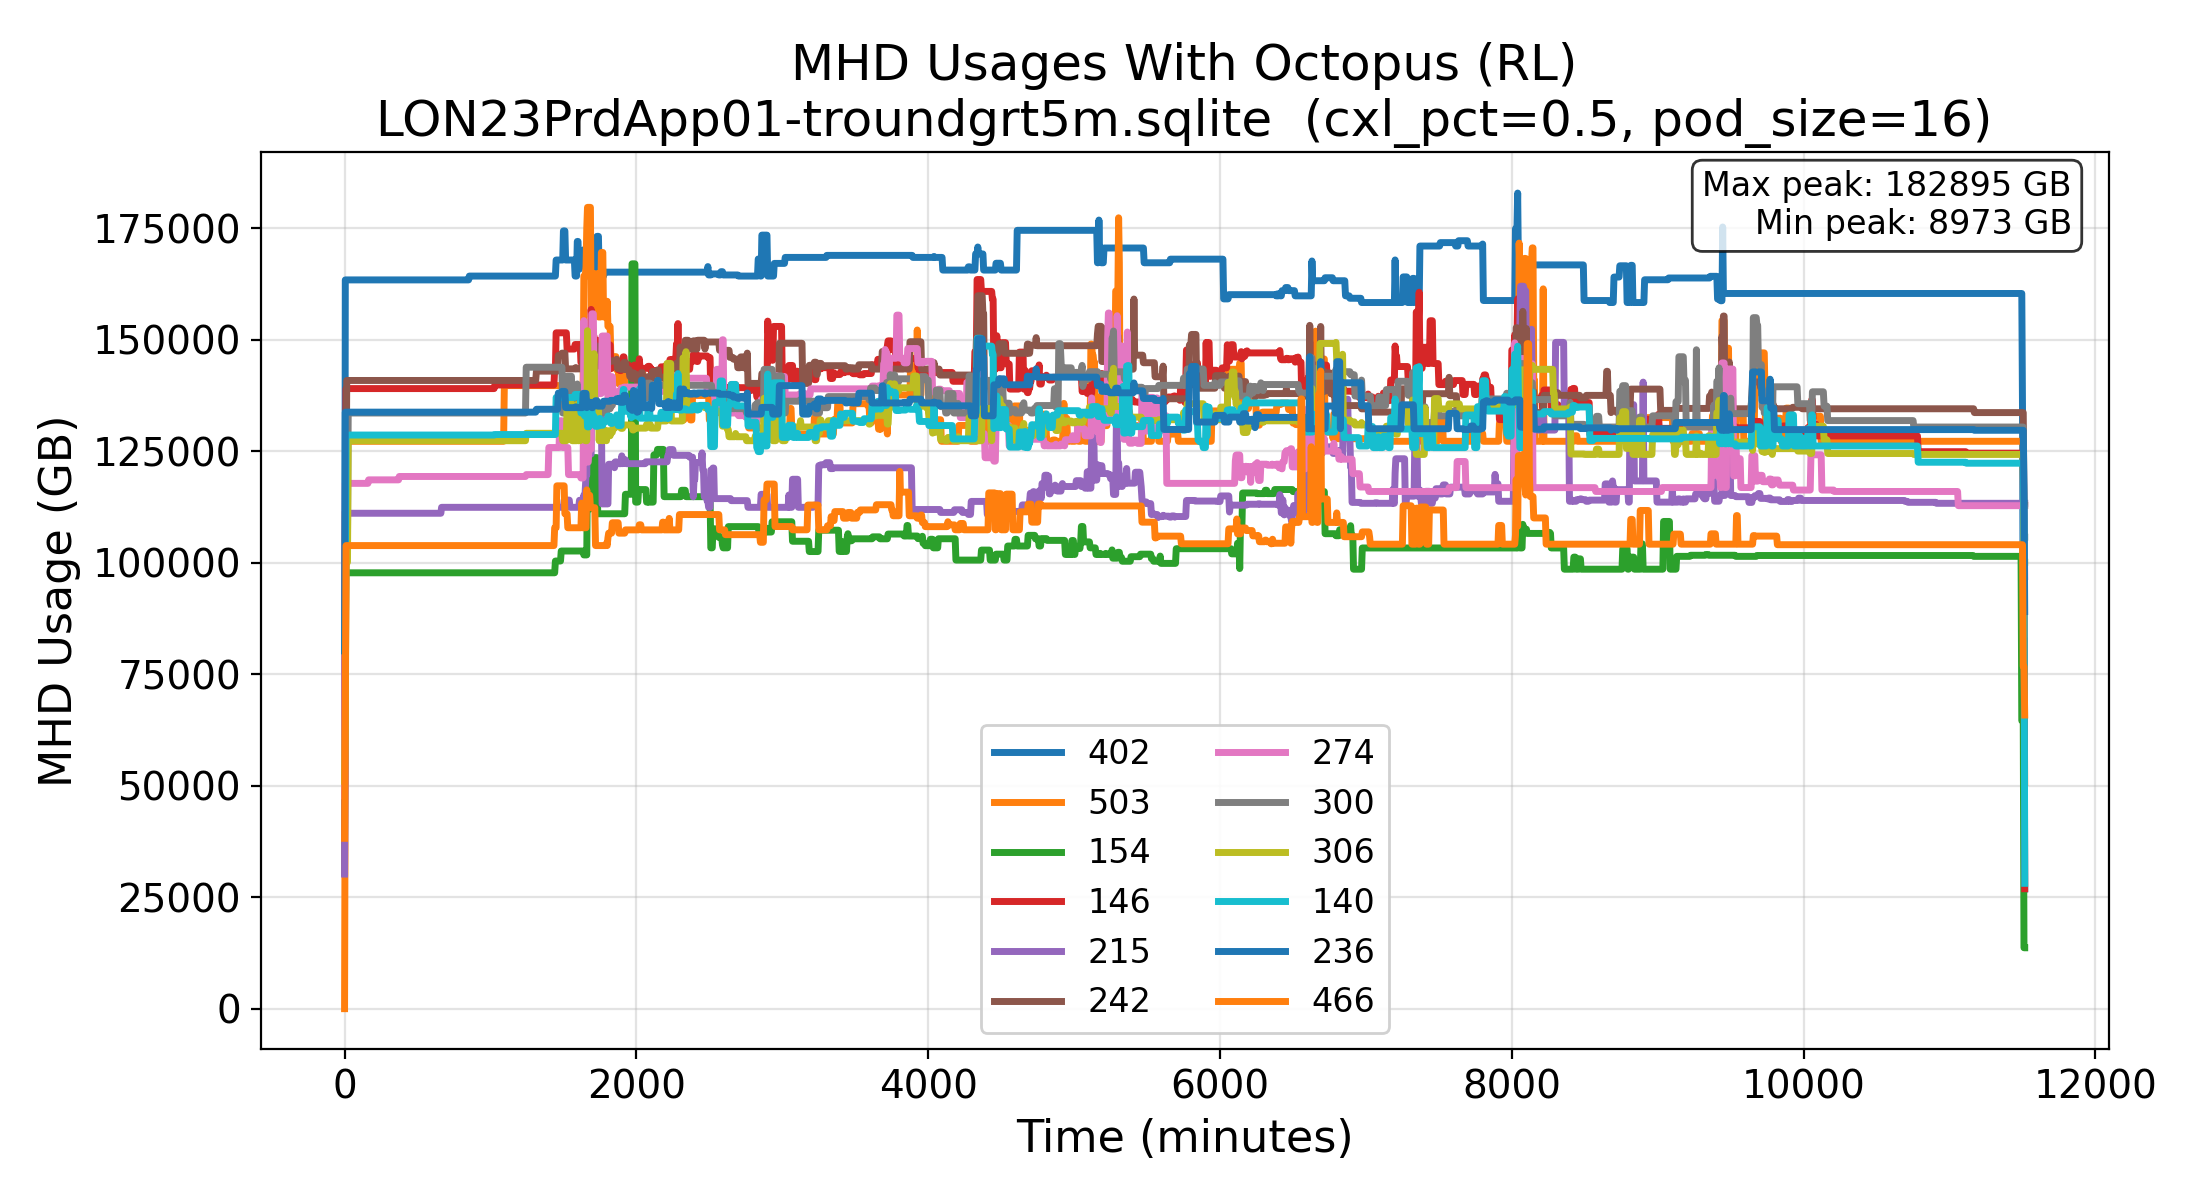
\includegraphics[width=\linewidth]{../v1/figs/mhd_timeseries_rl.png}
\end{minipage}
\caption{Existing comparison between greedy and the current SAC policy on the
same topology and trace family. The learned policy shows severe load collapse,
with roughly $20\times$ max/min imbalance, which is inconsistent with the
intended load-balancing objective.}
\label{fig:current_failure}
\end{figure}

The systems interpretation is straightforward: if the allocator cannot even keep
MPD load within a reasonable band, it is not yet solving the deployment problem
that Octopus cares about.

\section{Next Steps}

The next phase should be organized as a sequence of falsifiable experiments. Each
experiment must validate one diagnosis rather than bundling multiple changes into
a single opaque improvement claim.

\begin{enumerate}[leftmargin=*]
    \item \textbf{State ablation.} Compare the current observation against richer
    variants that add temporal deltas and future-pressure features such as
    short-term release, medium-term release, sticky load, and VM count per MPD.
    This validates whether the current failure is caused by missing observability
    of future headroom rather than by optimizer choice alone.

    \item \textbf{Reward ablation.} Compare peak-only reward, peak-plus-variance
    reward, and a fuller reward with direct over-capacity penalties and optional
    delayed components. This validates whether denser shaping aligns learning with
    pooling savings and reduces the current load-collapse behavior.

    \item \textbf{Training volume, curriculum, and domain randomization.} Sweep
    training budget from the current 1M-step regime to substantially larger runs,
    while adding staged curriculum learning and systematic randomization over
    traces, windows, pod mappings, and topology variants. This validates whether
    current failure is partly under-training or overfitting to a narrow offline
    setup.

    \item \textbf{SAC versus PPO in the offline setting.} Only after state and
    reward fixes are in place, compare SAC and PPO \cite{schulman2017ppo} as
    offline learners on the same held-out evaluation suite. This validates
    whether replay-buffer effects are a material contributor to poor
    generalization or whether the base task formulation remains the primary
    bottleneck.

    \item \textbf{LCPO only after offline success under online drift.} LCPO
    \cite{hamadanian2025lcpo} should be introduced only after an offline policy
    already achieves competent load balancing. The online experiment should then
    inject workload drift and continuous adaptation, measuring whether LCPO
    preserves older context behavior while adapting to new regimes. This
    validates deployment-time forgetting resistance rather than base-task
    learnability.
\end{enumerate}

Across all five steps, the minimum reporting set should include pooling savings,
worst-MPD peak, MPD imbalance, over-capacity events, and held-out
generalization.

\section{Detailed Results}

This section expands the current evidence one result at a time using a repeated
structure. The goal is to separate what the project already knows from what it
still needs to validate.

\subsection{Result 1: Real Traces Show Recoverable Pooling Headroom}

\paragraph{Setup.}
The project uses two weeks of Azure VM trace data from ten datacenters. Demand is
aggregated into cluster-level time series and compared against total installed
DRAM, using five-minute granularity in the existing analysis.

\paragraph{Measurement.}
The key measurement is the cluster-level peak-to-mean ratio, shown in
Figure~\ref{fig:motivation_peak_to_mean} and the broader demand visualization in
Figure~\ref{fig:detailed_demand}. The reported range is approximately
$1.13\times$ to $1.26\times$ across sites.

\paragraph{Interpretation.}
This is the foundational positive result. It shows that the memory-pooling
opportunity is not hypothetical: aggregate demand is smoother than the worst
server-local peaks, so there is real headroom to reclaim if allocation keeps the
pool balanced.

\paragraph{Limitation.}
This result does not say anything about whether the current learned policy can
realize the opportunity. It establishes the motivation for pooling, not the
effectiveness of the present allocator.

\begin{figure}[H]
\centering
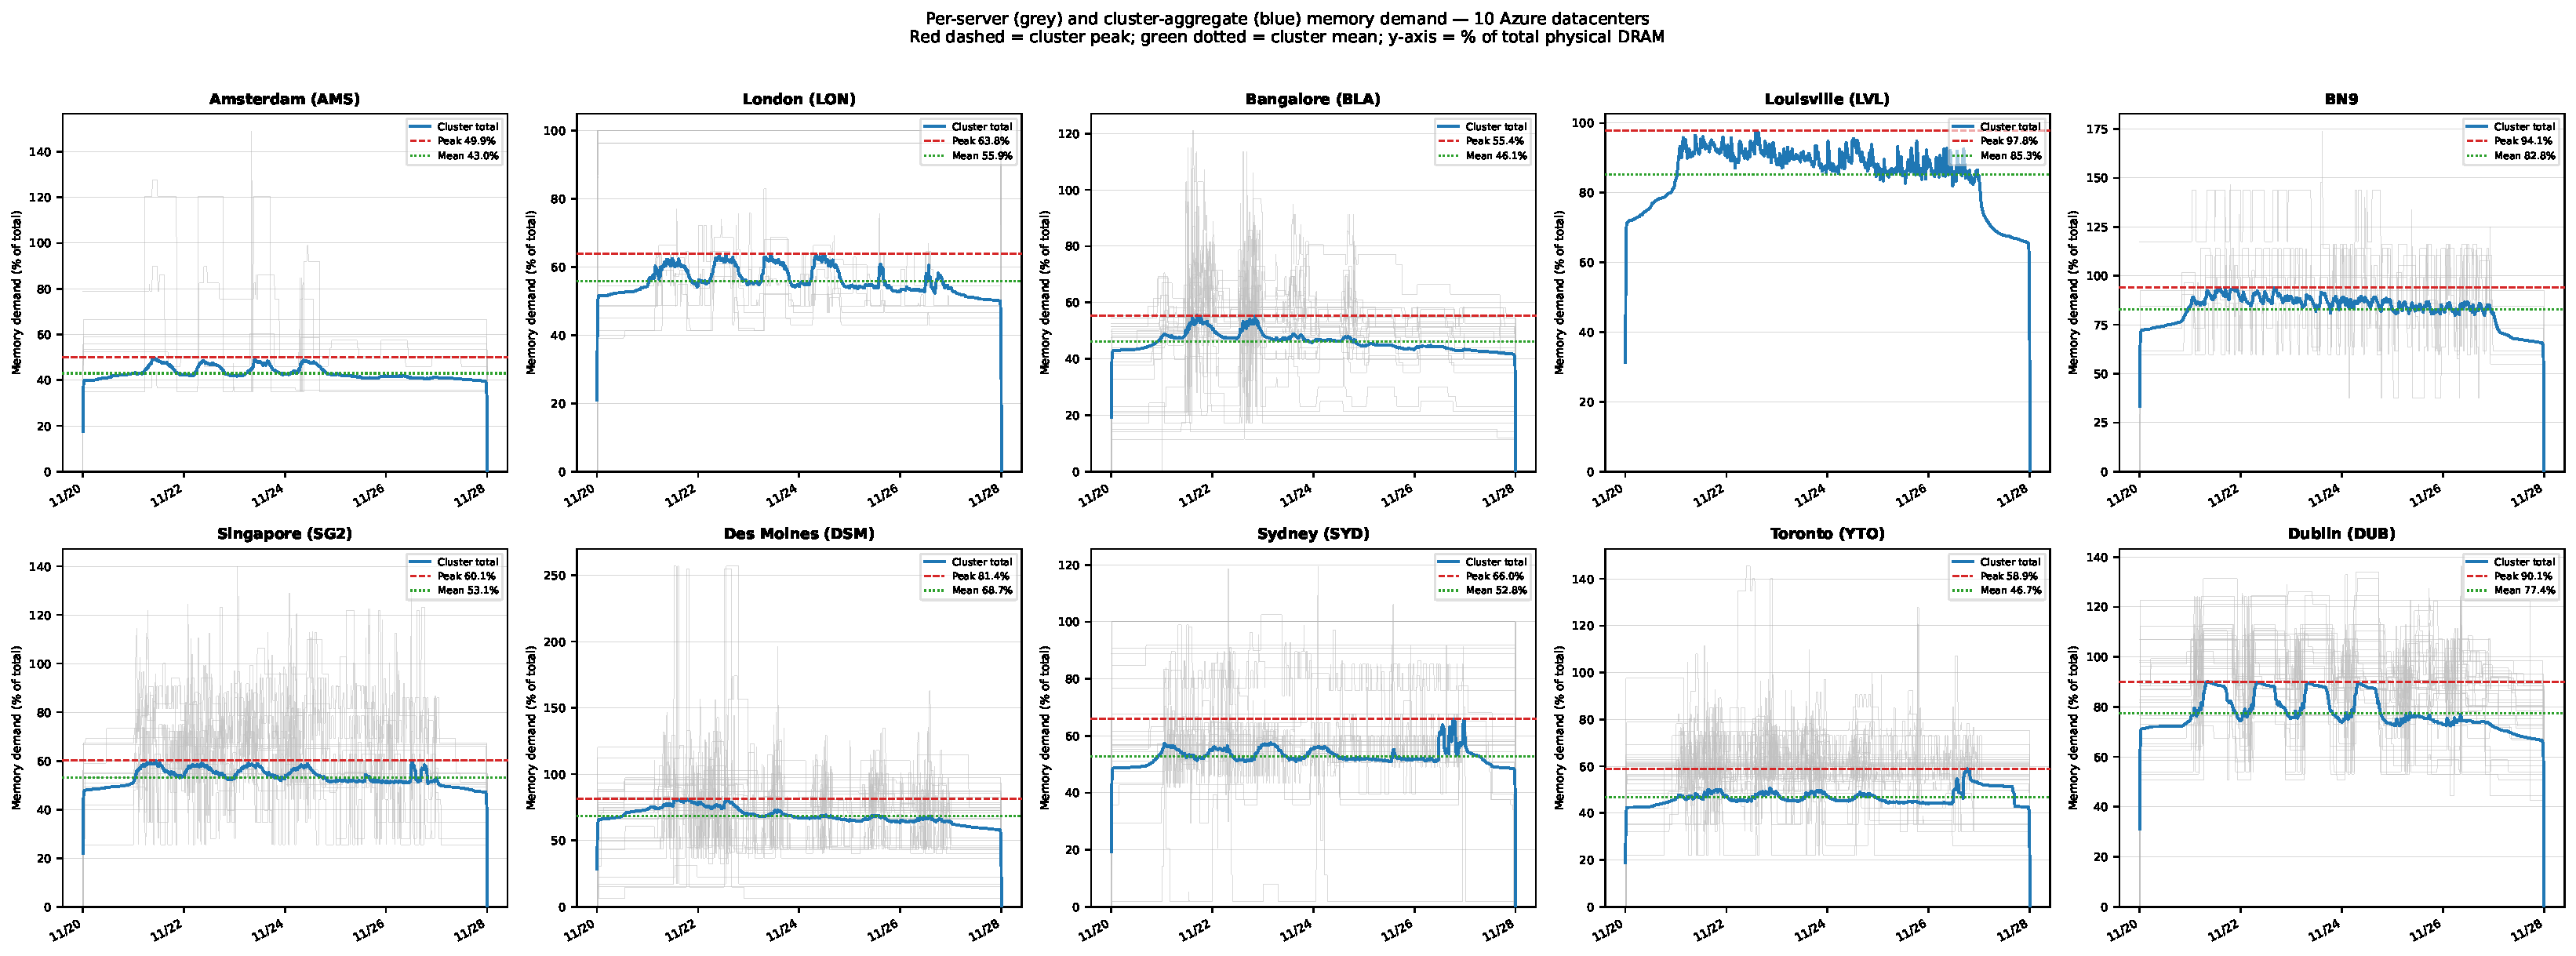
\includegraphics[width=\textwidth]{../v1/figs/demand_overview.pdf}
\caption{Existing demand overview from the Octopus analysis. The aggregate trace
is smoother than per-server traces, which is precisely the statistical structure
that makes pooling attractive.}
\label{fig:detailed_demand}
\end{figure}

\subsection{Result 2: Sparse Octopus Topology Is Harder Than Full Reachability}

\paragraph{Setup.}
The project compares fully-connected and sparse Octopus-style topologies under
the greedy baseline, sweeping pod size and CXL fraction in prior simulator runs.

\paragraph{Measurement.}
Prior simulator runs show that fully-connected topology consistently outperforms
sparse Octopus, with the gap widening as the CXL fraction grows.

\paragraph{Interpretation.}
This is the strongest topology result in the current materials. It confirms that
Octopus is not merely an implementation inconvenience layered over an easy
pooling problem. Sparse connectivity materially constrains placement quality,
which is exactly why a better allocator could matter.

\paragraph{Limitation.}
This result is based on baseline simulation behavior rather than the new learned
policy. It motivates learning, but it does not demonstrate that RL currently
closes the topology-induced gap.

\subsection{Result 3: Baselines Already Define a Meaningful Systems Target}

\paragraph{Setup.}
The current repository contains prior Octopus simulation summaries for heuristic
baselines and larger topology settings. These are not new RL wins, but they
establish the savings regime that a learned allocator must eventually reach or
improve upon.

\paragraph{Measurement.}
Table~\ref{tab:baseline_targets} summarizes three reference numbers used in the
current project narrative: a rough project break-even threshold of about $3\%$,
prior greedy savings of about $16\%$ on Acadia-96-style discussion points in the
project, and a simulator result of $26.3\%$ greedy savings on the
\texttt{random\_L96\_X8\_N4} topology.

\paragraph{Interpretation.}
The project is not trying to discover whether any pooling benefit exists. It is
trying to improve on already-meaningful baseline savings under realistic sparse
constraints. That gives the RL effort a concrete systems bar.

\paragraph{Limitation.}
These numbers come from prior project analyses and topology-specific runs, not
from the current SAC training pipeline. They should be treated as targets and
reference points rather than as evidence that the present learned policy is
competitive.

\begin{table}[H]
\centering
\small
\renewcommand{\arraystretch}{1.2}
\begin{tabular}{p{0.36\linewidth}p{0.18\linewidth}p{0.34\linewidth}}
\toprule
\textbf{Reference point} & \textbf{Value} & \textbf{Role in this report} \\
\midrule
Approximate project break-even threshold & $\sim 3\%$ & Minimum savings level at which pooling is economically interesting in the project discussion. \\
Prior greedy savings on Acadia-96-style project evidence & $\sim 16\%$ & Indicates that sparse pooling can already clear the economic bar comfortably. \\
Greedy savings on \texttt{random\_L96\_X8\_N4} & $26.3\%$ & Concrete simulator baseline showing that large sparse topologies can achieve substantial savings. \\
\bottomrule
\end{tabular}
\caption{Reference baseline targets drawn from the current project materials.
These numbers define the regime the learned allocator must eventually match or
beat.}
\label{tab:baseline_targets}
\end{table}

\subsection{Result 4: The Current Learned Policy Collapses Load Instead of Balancing It}

\paragraph{Setup.}
The current learner is SAC trained for 1M timesteps with the newer fast
configuration emphasized in the slide deck. Evaluation compares the resulting
policy against greedy on the same broad topology and trace setting.

\paragraph{Measurement.}
The strongest available failure signal is the MPD load pattern in
Figure~\ref{fig:current_failure}: the learned policy produces roughly
$20\times$ max/min imbalance, whereas greedy remains within a far narrower band.

\paragraph{Interpretation.}
This is the central negative result of the report. The policy is not merely
slightly worse than greedy; it appears to have learned behavior that is
incompatible with the systems objective. The most plausible causes, based on the
current notes, are sparse reward, missing future-pressure state, missing temporal
state, and insufficiently broad training.

\paragraph{Are we accounting for future reward?}
\textcolor{red}{Yes in the algorithmic sense, but not yet in the task-design sense. SAC learns a
critic (a value function) and optimizes expected discounted return with a high
discount factor ($\gamma \approx 0.999$ in the current training script). However,
the environment reward is currently a myopic proxy (an immediate $-\Delta$ peak
penalty at each VM arrival). When the reward does not explicitly reflect
long-horizon consequences (e.g., an allocation at midnight causing the true peak
at 9am), the value function can only propagate that same myopic signal forward.
This is exactly the credit-assignment gap motivating the planned reward redesign:
add denser immediate shaping (peak + variance + explicit over-capacity penalties)
and, if needed, add a delayed component keyed to VM termination to better
attribute lifetime impact.}

\paragraph{Limitation.}
The figure diagnoses behavior, not mechanism. It shows what went wrong, but it
does not by itself isolate whether reward design, state design, training budget,
or algorithm family is the dominant cause.

\subsection{Result 5: Current Proxy Training Metrics Do Not Yet Establish Robust Generalization}

\paragraph{Setup.}
The current training notes compare a slower SAC configuration against a faster
one, both run for 1M timesteps with evaluation on a held-out trace.

\paragraph{Measurement.}
The fast run reportedly reaches final evaluation reward around $-2.71$, compared
with about $-3.17$ for the slower run. At the same time, the fast run performs
far fewer gradient updates than the slow run.

\paragraph{Interpretation.}
Two conclusions follow. First, the faster configuration is operationally
preferable because it reduces wall-clock cost dramatically. Second, neither proxy
reward trend is enough to claim a good allocator, because the more important
systems metric remains pooling savings and the behavior-level evidence still shows
load collapse.

\paragraph{Limitation.}
Evaluation reward is only a proxy. Without consistent reporting of pooling
savings, imbalance, and over-capacity events during training and validation, it
is difficult to know whether the policy is improving in the way a systems paper
would ultimately care about.

\section{Conclusion}

The current Octopus effort already has a strong systems narrative. Real traces
show recoverable pooling headroom. Sparse topology makes the placement problem
non-trivial. The simulator and repeated-remapping evaluation loop already expose
meaningful behavior. What is missing is not motivation, but a policy that behaves
like a robust allocator.

The most important present result is therefore negative: the current SAC policy
shows severe load collapse and weak generalization. That failure should be used
constructively. It suggests a disciplined next phase centered on state ablation,
reward ablation, stronger training protocols, and offline SAC-versus-PPO
comparison before any LCPO deployment study. In short, the project should first
make Octopus memory allocation learnable offline, and only then tackle
deployment-time non-stationarity.

\bibliographystyle{plainnat}
\bibliography{../v1/references}

\end{document}
